\documentclass[10pt]{beamer}
%\usepackage{ngerman}
\usepackage{soul}
\usepackage{mathtools}
\usepackage{amssymb,amsmath,amsfonts}
\usepackage[utf8]{inputenc}
\usepackage{graphicx}
\usepackage{float}
\usepackage[autostyle=true,german=quotes]{csquotes}
\usepackage{gensymb}
\usepackage{units}
\usepackage{fancyhdr}
\usepackage[font=small,labelfont=bf]{caption}
\usepackage{wrapfig}
\usepackage{array}
\usepackage{subcaption}
\usepackage[export]{adjustbox}
\usepackage[absolute,overlay]{textpos}
\usepackage[english]{babel}
\usepackage{multicol}

\usepackage[%backend=biber,
citestyle=authortitle,
sorting=nty
]{biblatex}

\graphicspath{{./figures/}}
\addbibresource{../solensim.bib}

\setbeamertemplate{navigation symbols}{}
%\setbeamertemplate{bibliography item}{\insertbiblabel}
\setbeamertemplate{section in toc}[square]
\setbeamertemplate{subsection in toc}[square]
\setbeamertemplate{footline}[frame number]

\newcommand{\citesame}{$^{\thefootnote}$}
\newcommand{\citeprev}{\addtocounter{footnote}{-1}$^{\thefootnote}$\addtocounter{footnote}{1}}
\newcommand{\citepprev}{\addtocounter{footnote}{-2}$^{\thefootnote}$\addtocounter{footnote}{2}}
\newcommand{\bull}{$\bullet$}
\newcommand{\rarrow}{$\rightarrow$ }
\newcommand{\rfn}{\setcounter{footnote}{0}}
\newcommand{\tocslide}{
\begin{frame}
  \frametitle{Structure}
  \tableofcontents[currentsection]
\end{frame}
}

\title{Solenoid electron lenses}
\subtitle{Fundamentals and design}
\author{Anton Douginets \and Andrii Yanovets}
\date{22.06.2020}

\begin{document}
%Title slide:
\begin{frame}[plain]
  \titlepage
\end{frame}

%TOC slide:
\begin{frame}
  \frametitle{Structure}
  \tableofcontents%[currentsection]
\end{frame}

%%%%%%%%%%%%%
\section{Motivation}
%%%%%%%%%%%%%

\begin{frame}
  \frametitle{Motivation}
  \rfn
  \begin{itemize}
    \item Magnetic lenses - important components of particle accelerators, microscopes
    \item Electromagnet solenoids - physical foundation of more advanced magnetic lenses
    \item Design constraints:
    \begin{itemize}
      \item Power consumption
      \item Physical size, material usage
      \item Characteristic parameters for interaction with other machine components
    \end{itemize}
  \end{itemize}
  \begin{figure}
  \centering
    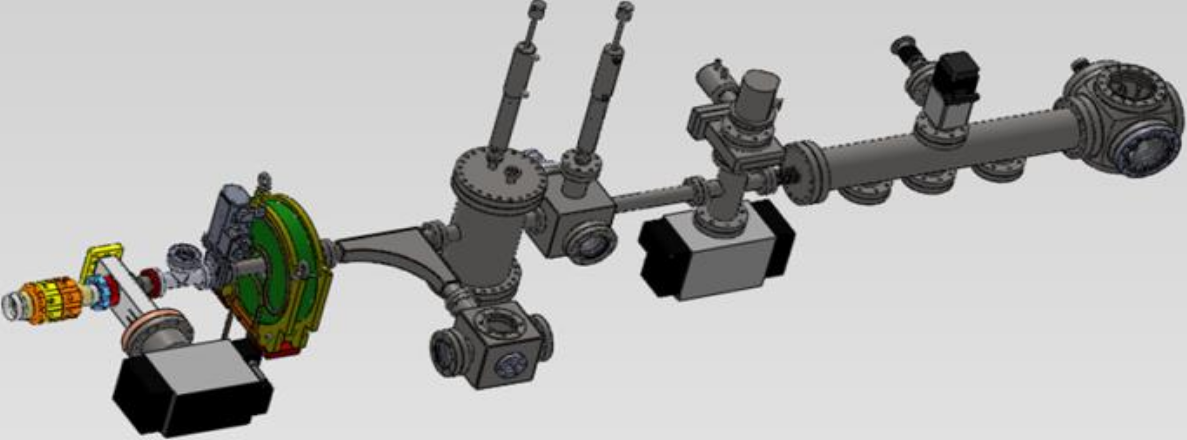
\includegraphics[width=0.7\textwidth]{AREAL}
    \caption{Schematic\footcite{Grigoryan2014} of AREAL, an electron bunch-research oriented linac\footcite{Grigoryan2011}}

  \end{figure}
\end{frame}

%%%%%%%%%%%%%
\section{Magnetic lens overview}
%%%%%%%%%%%%%
\tocslide
\subsection{General notions}
\begin{frame}
  \frametitle{Electron optics}
  \rfn
  \framesubtitle{Definition}
  \begin{table}[t]
    \centering
    \begin{tabular}{   m{5cm}  m{5cm}  }
    \underline{Classic optics} & \underline{Electron optics} \\
    & \\
    \bull Light ray - photons &  \bull Electron beam - electrons  \\
    & \\
    \bull Can pass through optically transparent solids  & \bull  Gets absorbed/loses energy due to interactions with atoms in media \\
    & \\
    \bull Bends due to refractive index difference between media & \bull  Bends due to Coulomb and Lorentz forces in the presense of external EM-fields \\
    \end{tabular}
  \end{table}
\end{frame}

\begin{frame}
  \frametitle{Magnet lenses}
  \framesubtitle{Requirements}
  \rfn
  A lens must have the following properties:
  \vspace{0.15cm}
  \begin{itemize}
    \item deflection increases with increasing deviation of the beam from the optic axis;
    \vspace{0.15cm}
    \item electron energy should not change, or change negligebly;
    \vspace{0.15cm}
    \item symmetry of deflection on all sides of the optical axis;
    \vspace{0.15cm}
    \item methods and laws of classical optics (such as thin lens formula and approximation, matrix formalism) are assumed to be applicable.
  \end{itemize}
\end{frame}

\begin{frame}
  \frametitle{Magnet lenses}
  \framesubtitle{Solenoids}
  \begin{figure}
    \subfloat[A solenoid with S as optical axis\footcite{a_optics}]{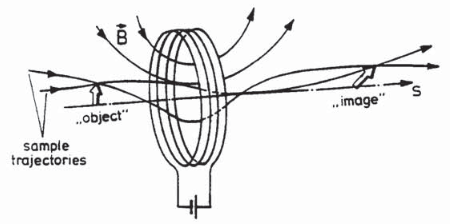
\includegraphics[width=0.5\textwidth]{Solenoid_scheme3.png}}
    \subfloat[Cross-section of a magnetic lens\footcite{Egerton}]{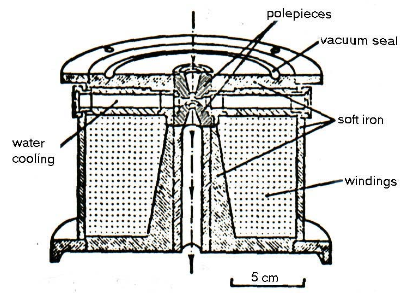
\includegraphics[width=0.5\textwidth]{Solenoid_pic1.png}}
    \label{some example}
  \end{figure}
\end{frame}

\begin{frame}
  \frametitle{Magnet lenses}
  \framesubtitle{Solenoids}
  \rfn
  \begin{figure}
    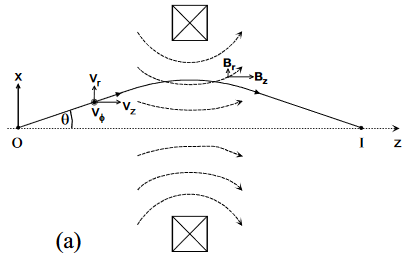
\includegraphics[width=.5\textwidth]{El_traj_in_B1.png}
    \caption{A solenoid cross-section along the optic axis\footcite{Egerton}}
  \end{figure}
  \begin{scriptsize}
  \begin{columns}
    \begin{column}{0.45\textwidth}
      \begin{equation}
        F_{\varphi}=e\left(B_{z}v_{r} - v_{z}B_{r}\right)
      \end{equation}
      \begin{equation}
        F_{r}=-e\left(v_{z}B_{z}\right)
      \end{equation}
      \begin{equation}
        F_{z}=e\left(v_{\varphi}B_{r}\right)
      \end{equation}
    \end{column}
    \begin{column}{0.55\textwidth}
      \begin{equation}
        \gamma m\left(\ddot{r}-r\dot{\varphi}^{2}\right)=-er\dot{\varphi}B_{z}
      \end{equation}
      \begin{equation}
        \gamma m\frac{d}{dt}\left(r^{2}\dot{\varphi}\right)=-er(\dot rB_{z}+B_{r}\dot{z})
      \end{equation}
      \begin{equation}
        \gamma m\ddot{z}=er\dot{\varphi}B_{r}
      \end{equation}
    \end{column}
  \end{columns}
  \end{scriptsize}
\end{frame}

\begin{frame}
  \frametitle{Magnet lenses}
  \framesubtitle{Electron path equations}
  \rfn
  \begin{scriptsize}
  \begin{columns}
    \begin{column}{0.6\textwidth}
      \begin{equation}
        B_{z}\left(z,r\right)=\underset{n}{\sum}\frac{\left(-1\right)^{n}}{n!n!}\left(\frac{r}{2}\right)^{2n}\frac{\partial^{2n}B_{z,\,axis}}{\partial z^{2n}}
      \end{equation}
      \begin{equation}
        B_{r}\left(z,r\right)=\underset{n}{\sum}\frac{\left(-1\right)^{n}}{n!\left(n-1\right)!}\left(\frac{r}{2}\right)^{2n-1}\frac{\partial^{2n-1}B_{z,\,axis}}{\partial z^{2n-1}}
      \end{equation}
    \end{column}
    \begin{column}{0.5\textwidth}
      \bull From (5) follows:
      \begin{equation}
        \dot{\varphi}=\frac{e}{2\gamma m}B_{z}
      \end{equation}
      \bull From (4) and (6) follows:
      \begin{equation}
        \ddot{r}=-\left(\frac{e}{2\gamma m}\right)^{2}rB_{z}^{2}
      \end{equation}
      \begin{equation}
        \ddot{z}=-\left(\frac{e}{2\gamma m}\right)^{2}r^{2}B_{z}B'_{z}
      \end{equation}
    \end{column}
  \end{columns}
  \begin{equation}
    \ddot{r}=r''\dot{z}^{2}\approx r''\left(\beta c\right)^{2}\Rightarrow r''=\left(\frac{e}{2p_{z}}\right)^{2}rB_{z}^{2}
  \end{equation}
  \begin{equation}
    -\frac{r'}{r}=\frac{1}{f}\underset{integrate\,(12)}{\Rightarrow}\frac{1}{f}=\left(\frac{e}{2p_{z}}\right)^{2}\intop_{-\infty}^{\infty}B_{z}^{2}dz\coloneqq\left(\frac{e}{2p_{z}}\right)^{2}F_{2}
  \end{equation}
  \end{scriptsize}
\end{frame}

\begin{frame}
  \frametitle{Magnet lenses}
  \framesubtitle{Magnetic field of solenoid}
  \rfn
  \vspace{-1cm}
  \begin{figure}
    \centering
    \subfloat[Single-wind solenoid\footcite{Disser}]{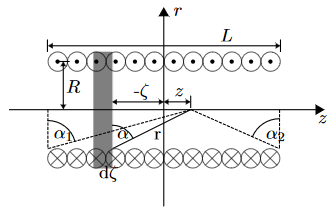
\includegraphics[width = 0.3\textwidth]     {Single_lay_solenoid2.png}}
    \hspace{0.1cm}
    \subfloat[Solenoid with multilayred windings\citesame]{\includegraphics[width = 0.3\textwidth]{Multilay_solenoid2.png}}
    %\hspace{0.1cm}
    \subfloat[Fields produced by two coils with same N and L=b]{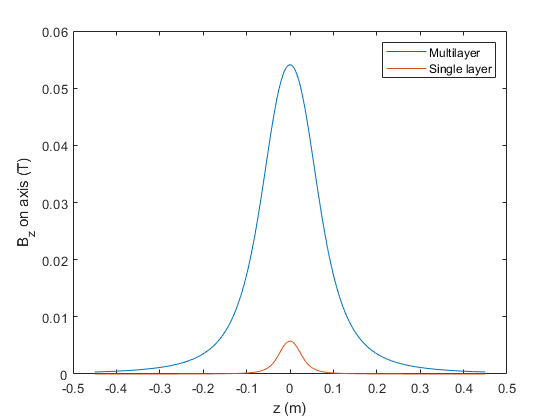
\includegraphics[width = 0.38\textwidth]{fieldcomparisson.png}}
    \label{some example}
  \end{figure}
  \begin{tiny}
  \begin{columns}
    \begin{column}{0.5\textwidth}
      Field of the solenoid (a):
      \begin{equation}
      B_{z}\!\left(z\right)=\!\frac{\mu_{0}nI}{2}\!\left(\!\frac{\triangle z}{\sqrt{R^{2}+\triangle z^{2}}}\!-\!\frac{\triangle z^{*}}{\sqrt{R^{2}+\triangle z^{*2}}}\!\right)\!
      \end{equation}
      \begin{equation}
      \triangle z=z-L/2
      \end{equation}
    \end{column}
    \begin{column}{0.6\textwidth}
      Approximate field of the solenoid (b)\citesame:
      \begin{equation}
        B_{z}\left(z\right)\approx\frac{\mu_{0}NI}{4}\left(\frac{Rc^{2}}{\left(z^{2}+Rc^{2}\right)^{3/2}}+\frac{Rc^{*2}}{\left(z^{2}+Rc^{*2}\right)^{3/2}}\right)
      \end{equation}
      \begin{equation}
        Rc=R_{sq}+c,\,R_{sq}=R_{m}\left(1+\frac{a^{2}}{24R_{m}^{2}}\right),\,c^{2}=\frac{b^{2}-a^{2}}{12}
      \end{equation}
    \end{column}
  \end{columns}
  \end{tiny}
\end{frame}

\subsection{Lens imperfections}

\begin{frame}
  \frametitle{Lens impefections}
  \rfn
  %\framesubtitle{Defects}
  \begin{small}
  There are 3 main limitations to consider when designing a solenoid lens:
  \begin{table}[t]
    \centering
    \begin{tabular}{   m{5cm}  m{5cm}  }
      &  \underline{Source:}\vspace{0.2cm} \\
      \bull Chromatic aberration & Spread of electron energies  \\
      & \\
      \bull RMS Emittance growth  &   Spread of eletron coordinates in position-and-momentum phase space \\
      & \\
      \bull Spherical aberration &  Real lens $\rightarrow$ different refraction based on distance from axis \\
    \end{tabular}
  \end{table}
  \end{small}
  \vspace{1cm}
  \begin{tiny}
  Emittance:
  \begin{equation}
    \epsilon_{n,rms}=\frac{1}{mc}\sqrt{\left\langle x^{2}\right\rangle \left\langle \tilde{p}_{x}^{2}\right\rangle -\left\langle x\tilde{p}_{x}\right\rangle ^{2}}=\frac{1}{mc}\left(\frac{e^{2}\sigma^{4}}{3\sqrt{2}p_{z,0}}F_{3}+\frac{e^{4}\sigma^{4}}{24\sqrt{2}p_{z,0}^{3}}F_{4}\right)
  \end{equation}
  Chromatic aberration:
  \begin{equation}
    r_{c}\approx\alpha f\left(\triangle E_{0}/E_{0}\right)\approx\alpha C_{c}\left(\triangle E_{0}/E_{0}\right)
  \end{equation}
  \end{tiny}
\end{frame}

\begin{frame}
  \frametitle{Lens impefections}
  \framesubtitle{Spherical aberration\footcite{Egerton}}
  \rfn
  \begin{columns}
    \begin{column}{0.4\textwidth}
      \begin{tiny}
      \begin{equation}
        \triangle f=c\cdotp x^{2}
      \end{equation}
      \begin{equation}
        x\approx f\cdotp tan\left(\alpha\right)
      \end{equation}
      \begin{align}
        r_{s}&=\triangle f\cdotp tan\left(\alpha\right)\approx c\cdotp f^{2}tan\left(\alpha\right)^{3}\\
        &=C_{s}\cdotp\left(\frac{r_{in}}{f-\frac{C_{s}r_{in}^{2}}{f^{2}}}\right)^{3}
      \end{align}
      \begin{equation}
        F_{3}=-\int\frac{B_{z}B''_{z}}{2}dz
      \end{equation}
      \begin{equation}
        F_{4}=\int B_{z}^{4}dz
      \end{equation}
      \end{tiny}
    \end{column}
    \begin{column}{0.6\textwidth}
    \begin{figure}[R]
      %\vspace{-1.5cm}\hspace{4cm}
      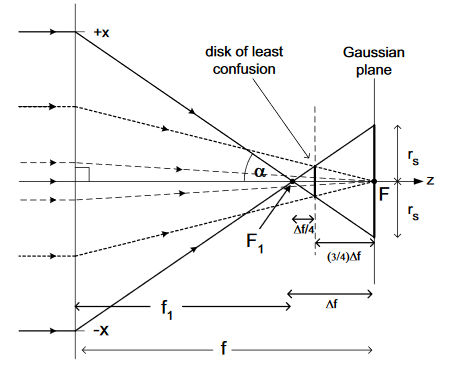
\includegraphics[width=\textwidth]{Spher_Abb1.png}
      %\begin{tiny}
      %\footcite{Egerton}}
      %\end{tiny}
    \end{figure}
    \end{column}
  \end{columns}
  \begin{columns}
    \begin{column}{0.6\textwidth}
    \vspace{-1cm}
    \begin{tiny}

        \begin{align}
          C_{s}&=\frac{e}{96m\tilde{U}}\int\left(\frac{2e}{m\tilde{U}}B_{z}^{4}+5\left(B_{z}'\right)^{2}-B_{z}B_{z}''\right)R^{4}dz \\
          &=\frac{e^{2}R^{4}}{4p_{z,0}^{2}}F_{3}+\frac{e^{4}R^{4}}{12p_{z,0}^{4}}F_{4}
        \end{align}
    \end{tiny}
    \end{column}
    \begin{column}{0.4\textwidth}
      \begin{figure}
      \caption{Illustration of beam radius change due to spherical aberration}
      \end{figure}
      \end{column}
  \end{columns}
  \end{frame}

%%%%%%%%%%%%%%%%%
\section{Project methodology}
%%%%%%%%%%%%%%%%%
\tocslide
\subsection{Aim}
\begin{frame}
  \rfn
  \frametitle{Project task}
  Simple solenoid lens design:
  \begin{itemize}
    \item Monochromatic \textit{e} beam, fixed beam radius $R$
    \item Target FWHM, peak $B_z$, $f$
    \item Optimize geometry, current for minimal spheric aberration
  \end{itemize}
  \begin{figure}
    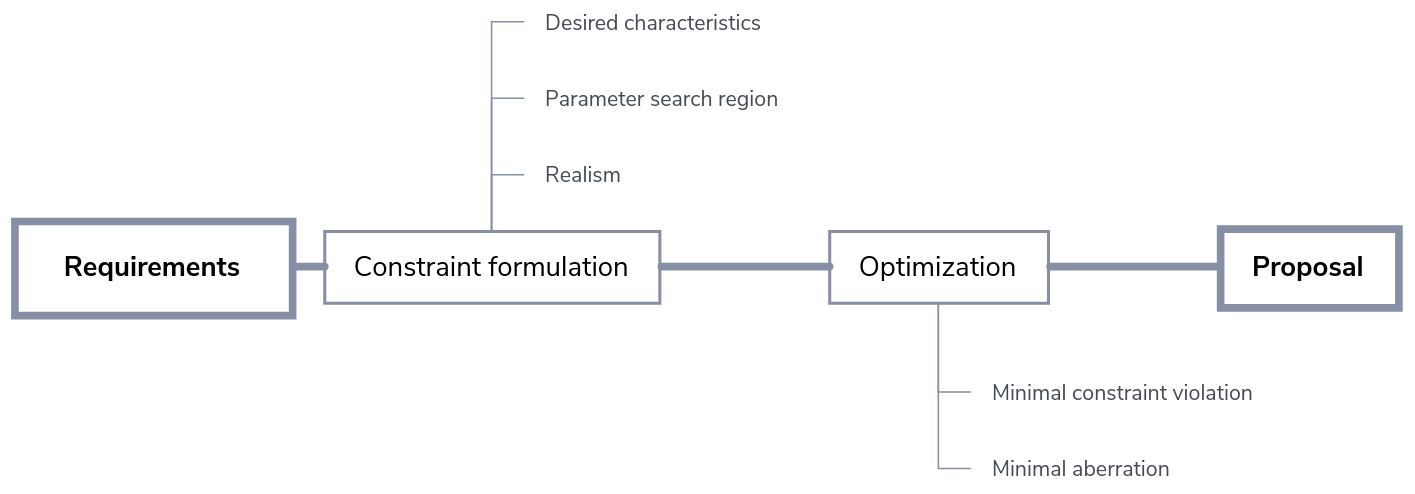
\includegraphics[width=\textwidth]{blok_cxema}
    \caption{Generalized design process}
  \end{figure}
\end{frame}

\subsection{Model}
\begin{frame}
  \rfn
  \frametitle{Solenoid model}
  \begin{itemize}
    \item Rectangular cross-section solenoid\footcite{Disser}
  \end{itemize}
  \begin{columns}
    \begin{column}{0.6\textwidth}
      Two-loop field approximation:
      \begin{small}
      \begin{center}
        \[
        B_{z}\left(z\right)\approx\frac{\mu_{0}NI}{4}\left(\frac{Rc^{2}}{\left(z^{2}+Rc^{2}\right)^{3/2}}+\frac{Rc^{*2}}{\left(z^{2}+Rc^{*2}\right)^{3/2}}\right);
        \]
        \[
        Rc = R_{sq}+c,\ \text{where}\
        c^{2} = \frac{b^{2}-a^{2}}{12},
        \]
        \[
        R_{sq} = R_{m}\left(1+\frac{a^{2}}{24R_{m}^{2}}\right).
        \]
      \end{center}
      \end{small}
    \end{column}
    \begin{column}{0.4\textwidth}
      \begin{figure}
        \centering
        \includegraphics[width=\textwidth]{figures/Multilay_solenoid2}
        \caption{Solenoid geometry:\\
        $R_m$ - mean radius\\
        $a$ - transverse width\\
        $b$ - axial length
        }
      \end{figure}
    \end{column}
  \end{columns}
  \vspace{0.25cm}
  Parameters: geometry, scaling factor $N\cdot I$ [Ampere-Turns]
\end{frame}

\begin{frame}
  \rfn
  \frametitle{Field integrals}
  For an axial beam, only the on-axis $B_z$ is of significance\footcite{Disser}. The field's optical properties are described in terms of:
  \begin{columns}
    \begin{column}{0.5\textwidth}
      \begin{center}
      \begin{small}
        \[F_1 = \int B_z dz\]
        \[F_2 = \int B_z^2 dz\]
      \end{small}
      \end{center}
    \end{column}
    \begin{column}{0.5\textwidth}
      \begin{center}
      \begin{small}
      \[F_3 = \int - \frac{B_z''\cdot B_z}{2} dz \]
      \[F_4 = \int B_z^4 dz\]
      \end{small}
      \end{center}
    \end{column}
  \end{columns}
  \vspace{1cm}
  whereas the integration domain is ($-\infty,\infty$).
\end{frame}

\begin{frame}
  \rfn
  \frametitle{Solenoid characteristics}
    \begin{itemize}
      \item Peak $B_z = B_z(0)$;
      \item Effective field length $\rightleftarrows$ FWHM
      \item Focal length:\\
      \begin{small}
        \[
        f = \left(\frac{2p_z}{e}\right)^2\frac{1}{F_2}
        \]
      \end{small}
      \item Aberration coefficient:\\
      \begin{small}
        \[
        c_s = \frac{e^{2}R^{4}}{4p_{z,0}^{2}}F_{3}+\frac{e^{4}R^{4}}{12p_{z,0}^{4}}F_{4}
        \]
      \end{small}
    \end{itemize}
    \vspace{0.5cm}
    Considerations:
    \begin{itemize}
      \item Geometry - size, material usage
      \item Scaling factor - power, material usage
      \item $f$, FWHM, $c_s$: interaction with other components, fitness to purpose
    \end{itemize}
\end{frame}

\subsection{Optimization}
\begin{frame}
  \frametitle{Optimization}
  \begin{itemize}
    \item Constrained Trust Region algorithm\footcite{scipyctr}:\\
      Iterative gradient search process; minimize merit function $m(p)$ of parameters $p = (s, R_m, a, b)$:
      \[
      m(p) = c_s(p) + k \cdot |\text{C}(p)|_2,\ \ \Delta p \leq R_T;
      \]
      C$(p) = (\text{C}_1,\text{C}_2,...,\text{C}_n)(p)$ - measure of constraint violation;
    \item Interior Point Algorithm\footcite{sqp}:\\
    Solves a sequence of approximate optimization problems, by transforming the original problem $\underset{x}{min}\,f\left(x\right),\:h\left(x\right)=0\wedge g\left(x\right)\leq0$ into $\underset{x}{min}\,f\left(x\right)=\underset{x,s}{min}\,f\left(x\right)-\mu\underset{i}{\sum}ln\left(s_{i}\right),\:h\left(x\right)=0\wedge g\left(x\right)+s=0$.
  \end{itemize}
  \vspace{-0.34cm}
  \begin{figure}
    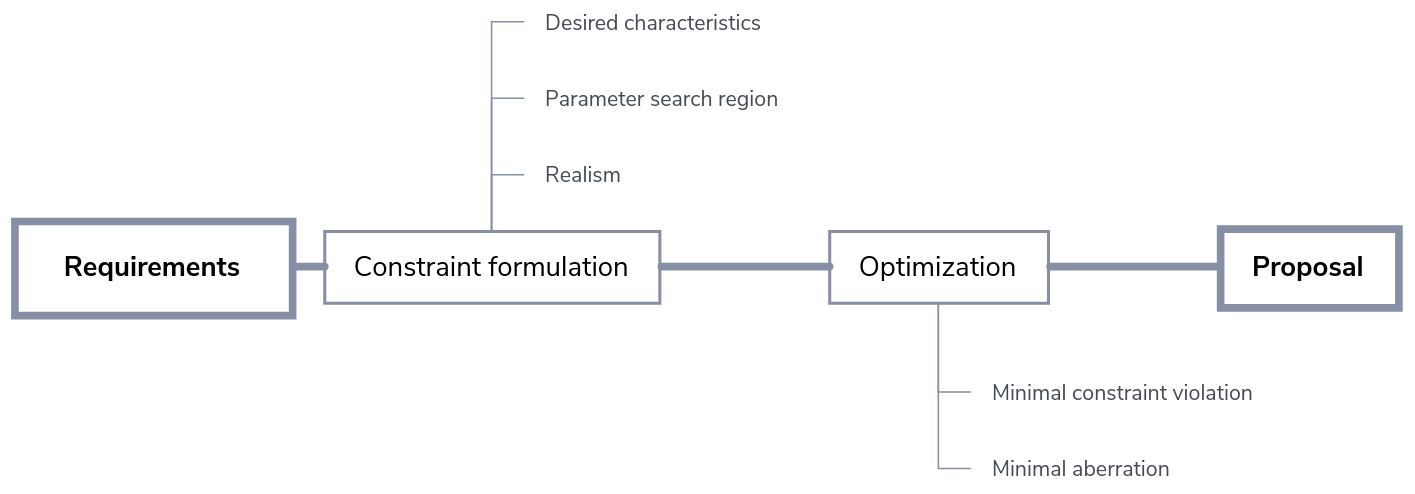
\includegraphics[width=0.8\textwidth]{blok_cxema}
  \end{figure}

\end{frame}

%%%%%%%%%%%%%%%%%
\section{Software demo}
%%%%%%%%%%%%%%%%%


\begin{frame}
  \frametitle{Interior point Algorithm results}
  \rfn
  \framesubtitle{Retrieved parameters}
    \begin{figure}
    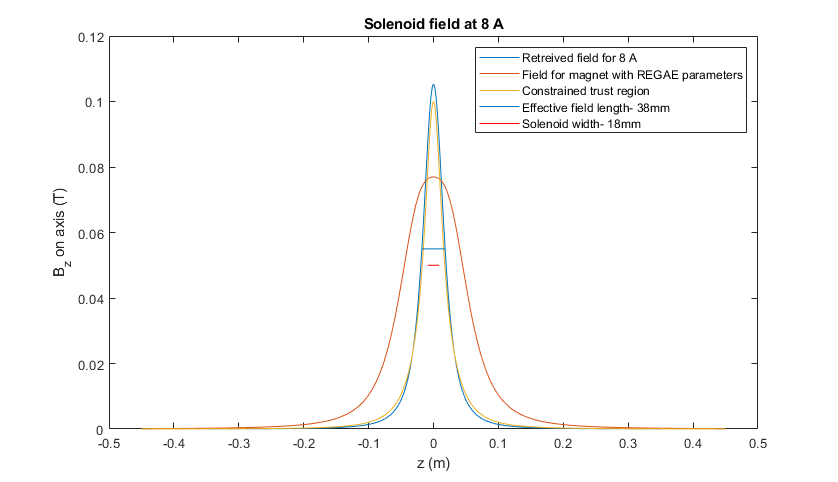
\includegraphics[width=.8\textwidth]{retreivedBz.png}
  \end{figure}
    \begin{tiny}
    \begin{table}[t]
    \centering
    \begin{tabular}{    m{1.4cm}|| m{0.9cm}| m{0.9cm} | m{1.2cm}| m{1.1cm}| m{1.5cm}| m{1.5cm}}
    & \underline{Height $a$ mm} & \underline{Width $b$ mm}& \underline{Max field $ B_z$ mT}& \underline{F. length $f$ cm}& \underline{Spherical ab. $C_s$ }& \underline{RMS emi. $\epsilon_{n.rms}$ } \\
    Opt. parameters    &17.6 & 17.6 &105& 50   &$1.7e-9 m$   &$3.4e-10 m$\\
    REGAE\footcite{Disser} & 99.5 & 41.8&79  & 30.5&$6.3e-11 m$ &$7.9e-11 m$\\
  \end{tabular}
  \end{table}
    \end{tiny}
\end{frame}

\begin{frame}
  \frametitle{Interior point Algorithm results}
  \rfn
  \framesubtitle{$F_3$ Integral}
  \begin{figure}
    \centering
    \subfloat[]{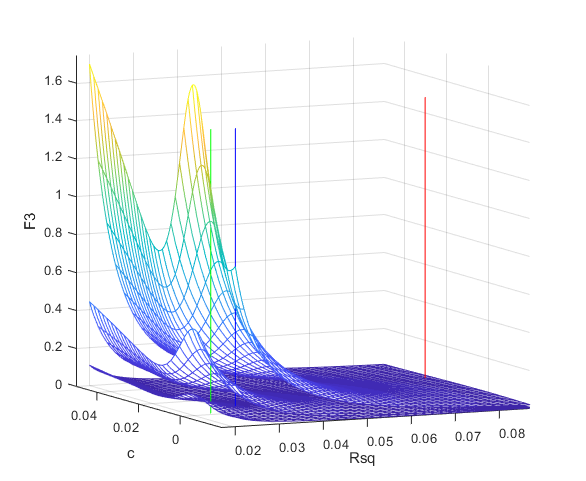
\includegraphics[width = 0.5\textwidth]     {F3.png}}
    \subfloat[]{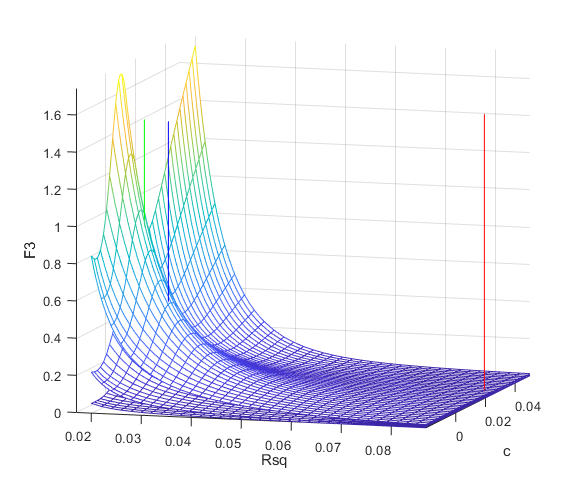
\includegraphics[width = 0.5\textwidth]{F33.png}}
    \label{some example}
    \caption{$F_3$ integral}
  \end{figure}
\end{frame}

%%%%%%%%%%%%%%%%%
\section{Summary, perspective}
%%%%%%%%%%%%%%%%%

\begin{frame}
  \frametitle{Perspective}
  \framesubtitle{Potential for further development}
  \rfn
  \framesubtitle{Subtitle}
\end{frame}

\begin{frame}
  \frametitle{Summary}
  \rfn
  \framesubtitle{Subtitle}
\end{frame}

\begin{frame}
  \frametitle{}
  \textbf{Thank you for your attention!}
\end{frame}

\begin{frame}[allowframebreaks]
  \frametitle{References}
  \printbibliography
\end{frame}

\end{document}
